\documentclass[red]{beamer}

\usetheme{default}

\setbeamertemplate{navigation symbols}{} 

\usepackage{amsfonts}
\usepackage{amsmath}
\usepackage{amsthm}
\usepackage{amssymb}
\usepackage{graphicx}

\usepackage[american]{babel}
\usepackage{csquotes}
\usepackage[style=apa,natbib=true,backend=biber]{biblatex}
\DeclareLanguageMapping{american}{american-apa}
\addbibresource{Polarization.bib}
% smaller references
\renewcommand*{\bibfont}{\scriptsize}

\usepackage{hyperref}
\ExecuteBibliographyOptions{doi=false}
\newbibmacro{string+doi}[1]{%
  \iffieldundef{doi}{#1}{\href{http://dx.doi.org/\thefield{doi}}{#1}}}
\DeclareFieldFormat{title}{\usebibmacro{string+doi}{\mkbibemph{#1}}}
\DeclareFieldFormat[article]{title}{\usebibmacro{string+doi}{\mkbibquote{#1}}}

%\logo{\includegraphics[height=0.6cm]{yourlogo.eps}}
%

\title[Polarization and Tasks]{Tasks and Work Force Polarization}
\author{Alex Cooper}
\date{7 June 2013}

\setlength{\itemsep}{\fill}

\begin{document}
%
\begin{frame}
\titlepage
\end{frame}
%
\section{International Experience}
\subsection{}

\begin{frame}[t]{United States}
\frametitle{U.S. wage inequality has risen since the 1960s}
\begin{center}
  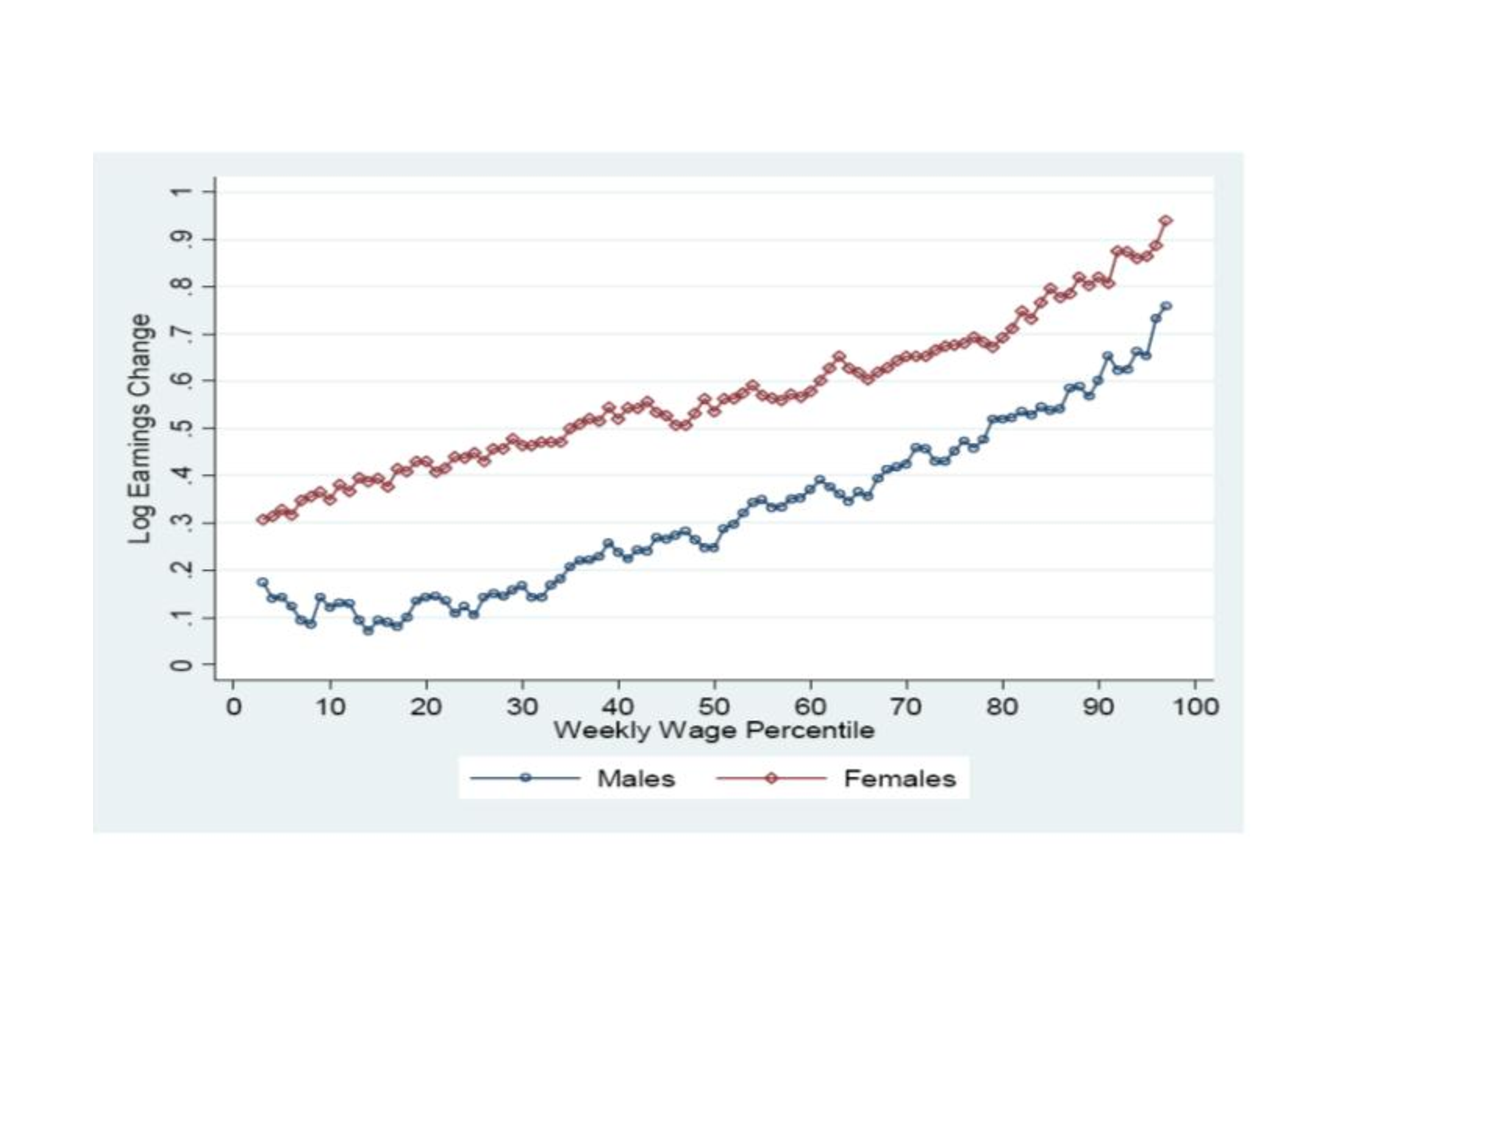
\includegraphics[width=\textwidth]{slides_fig/katz_kearney_2008_log_e_chg.pdf}
  \\
  Change in Log Real Weekly Wage by Percentile, Full-Time Workers, 1963-2005
  \citep{Autor2008}
\end{center}
\end{frame}

\begin{frame}
\frametitle{The `Canonical Model:' Skill-Based Technical Change}
\begin{itemize}
\item Model features:
\begin{itemize}
\item Two kinds of labor, high-skill ($H$) and low-skill ($L$).
\item $H$ and $L$ are different, and imperfect productive substitutes.
\item Technology \emph{factor-augmenting}: raises productivity/wages.
\item Wages set on the demand curve.
\end{itemize}
\vspace{5mm}
\item Production function representation:
\begin{equation*}
  \label{eq:cobbdoug}
  F(L,H) = \left[\left(A_LL\right)^{\frac{\sigma - 1}{\sigma}}
            + \left(A_HH\right)^{\frac{\sigma - 1}{\sigma}}
          \right]^\frac{\sigma}{(\sigma-1)}
\end{equation*}
\vspace{5mm}
\item If $\sigma>1$, ($H$, $L$ substitutes), SBTC implies rise in $A_H/A_L$.
\end{itemize}
\end{frame}

\begin{frame}
\frametitle{The `Canonical Model:' Skill-Based Technical Change}
\begin{itemize}
\item Predicts
  \begin{itemize}
  \item Increasing inequality, driven by skill demand.
  \item Rising college/education premium.
  \item Monotone wage growth in skills.
  \end{itemize}
\vspace{1cm}
\item Empirically successful, e.g.
  \begin{itemize}
  \item \citet{Katz1992}
  \item \citet{Card2001}
  \end{itemize}
\end{itemize}
\end{frame}

\begin{frame}[t]{International Evidence}
\frametitle{International evidence of non-monotone wage growth}
\begin{center}
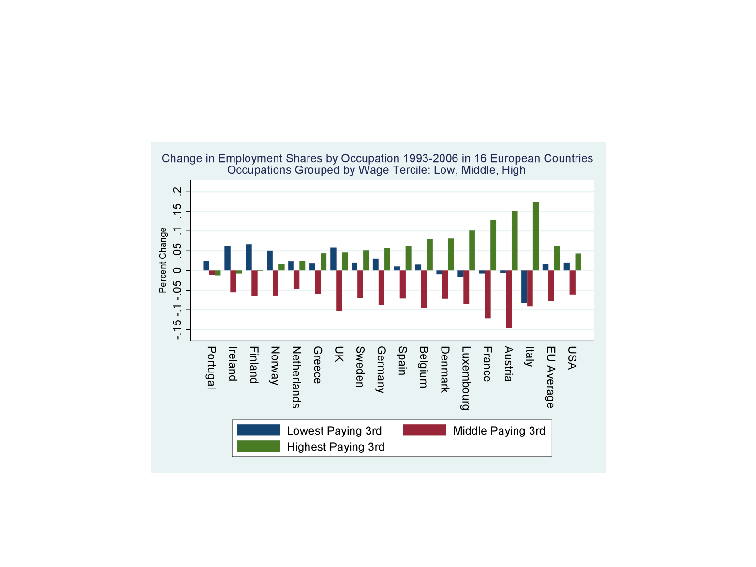
\includegraphics[width=0.9\textwidth]{slides_fig/international_nonmonotone.pdf}
\\
Wage growth by occupational wage tercile, 16 European countries \citep{Acemoglu2011}
\end{center}
\end{frame}

\begin{frame}[t]{United States}
\frametitle{Non-monotone employment growth (USA)}
\begin{center}
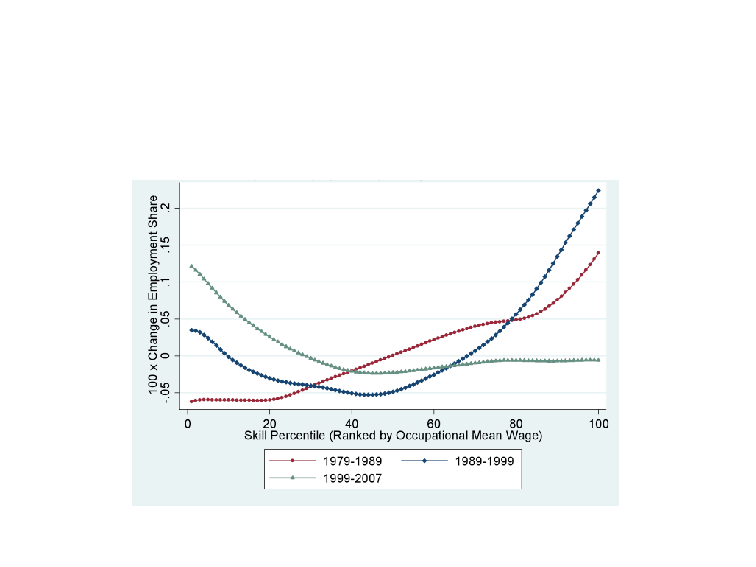
\includegraphics[width=\textwidth]{slides_fig/emp_occ_skill_percentile.pdf}
\\
Smoothed changes in employment by occupational skill percentile, 1979-2007
\citep{Acemoglu2011}
\end{center}
\end{frame}

\section{Alternative Model}
\begin{frame}[fragile] % Notice the [fragile] option %
\frametitle{\cite{Levy2003}}
``The skill content of recent technological change: An empirical exploration.'' \emph{The Quarterly Journal of Economics}, 118(4), 1279--1333.
\vspace{1cm}

\begin{itemize}
\item `Canonical' approach: factors produce output:
\[ K,L \overset{F(\cdot)}{\longrightarrow} Y. \]
\item ALM: factors produce tasks, which produce output:
\[ K, L \longrightarrow \text{tasks} \longrightarrow Y. \]
\end{itemize}
\end{frame}

\begin{frame}
\frametitle{The Task Approach}
\begin{itemize}
\item Jobs have different \emph{task content}, so technology can be factor-augmenting or a substitute.
\item Real cost of computing capital and machinery dramatically falling.
\item Capital can substitute for only certain `routine' tasks.
\item Model:
  \begin{itemize}
  \item Two kinds of tasks: routine ($L_R$), and non-routine ($L_N$). Capital $C$ and $L_R$ perfectly substitutable:
    $$ F(R,N) = (L_R + C)^{1-\beta}L_N^{\beta},\quad\beta\in(0,1)$$
  \item Workers are endowed with fixed `skills'
  \item Workers choose tasks they will supply endogenously
  \end{itemize}
\item Predictions: non-routine employment and wage growth exceeds that of routine employment
\end{itemize}
\end{frame}

\begin{frame}
  \frametitle{Job Polarization: United States}
  \begin{center}
  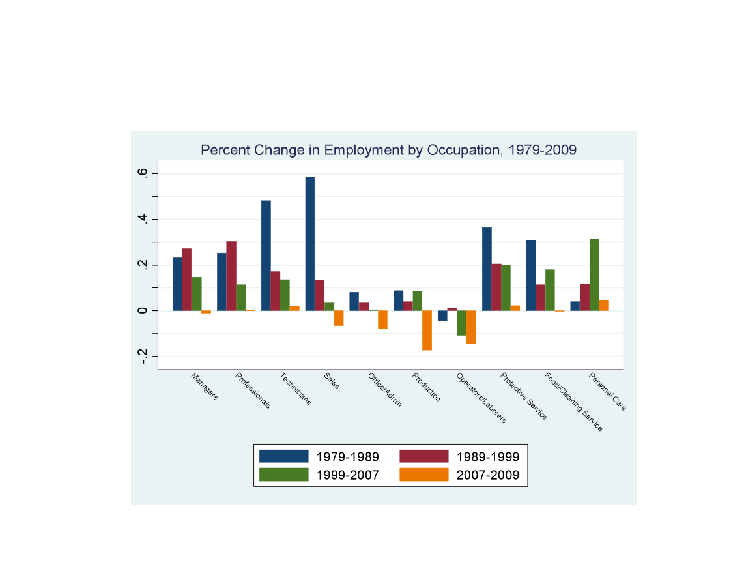
\includegraphics[width=0.9\textwidth]{slides_fig/level_by_occ.pdf} \\
  Percentage change in employment level, by occupation group, USA, 1979-2009 \citep{Acemoglu2011}
  \end{center}
\end{frame}

\begin{frame}
  \frametitle{Income growth, Australia, 1981-82 to 2007-08}
  \begin{center}
  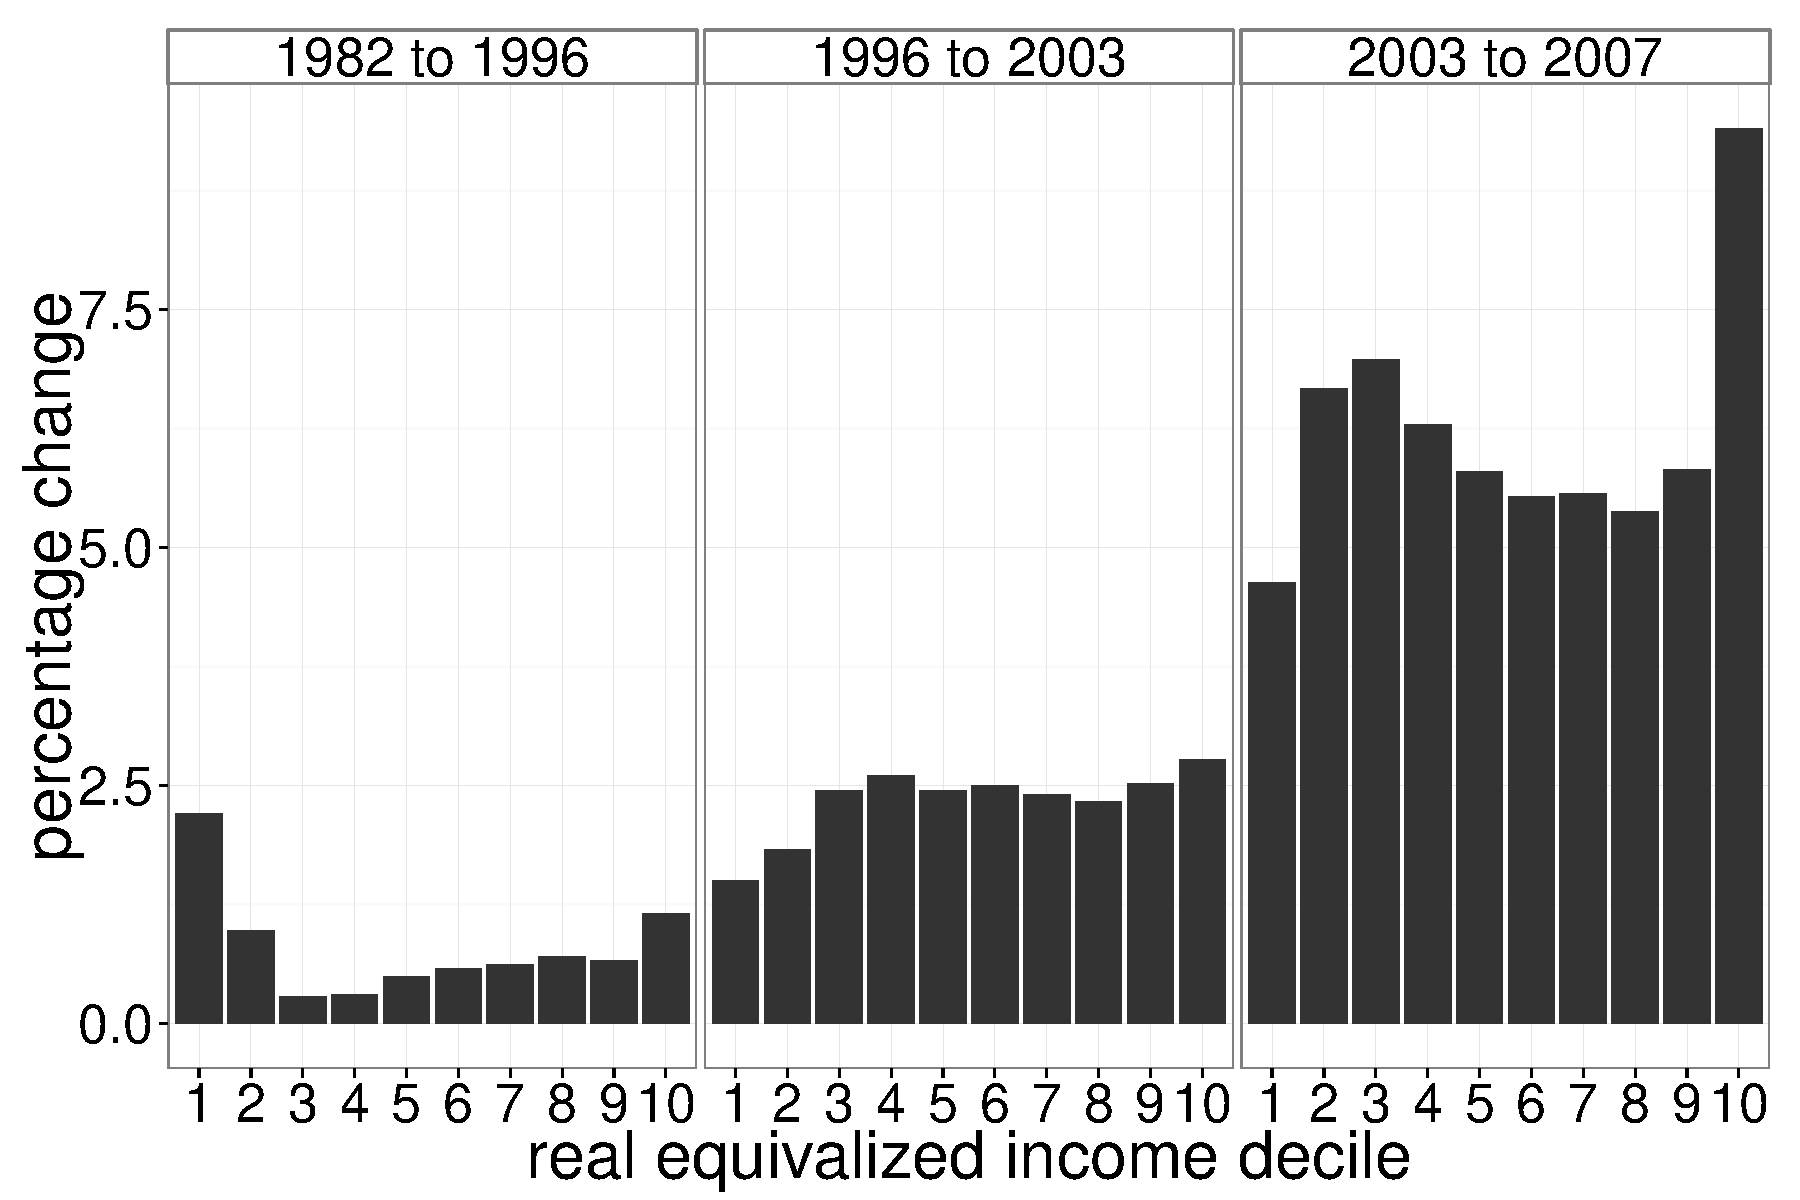
\includegraphics[width=0.9\textwidth]{slides_fig/figure_wage_deciles.pdf} \\
  Average annual percentage change in real equivalent income, working age (Whiteford, 2012)
  \end{center}
\end{frame}

\begin{frame}
  \frametitle{This Project: Questions}
  \begin{enumerate}
  \item  Has employment in Australia polarized in terms of routine and non-routine tasks as it has overseas?
    \begin{itemize}
    \item If not, why is Australia special?
    \end{itemize}
    \vspace{1cm}
  \item Does ICT capital investment explain this trend?
  \end{enumerate}
\end{frame}

\begin{frame}
  \frametitle{Data}
  \begin{enumerate}
  \item O*NET: Occupational task database
    \begin{itemize}
    \item Developed by US Department of Labor
    \item Details work activities by occupation
    \end{itemize}
    \vspace{10pt}
  \item David Autor's work type data categories
    \begin{itemize}
    \item Routine/non-routine and `off-shoreable'
    \end{itemize}
    \vspace{10pt}
  \item Australian Bureau of Statistics: Employment, Wages, Capital Investment
    \begin{itemize}
    \item Labor Force Survey (LFS)
    \item Survey of Income and Housing
    \item Census of Population and Housing
    \item National accounts: ICT and Machinery investment, capital stock
    \end{itemize}
  \end{enumerate}
\end{frame}

\begin{frame}
  \frametitle{Imputing Worker Activities from O*NET}
ABS data: $N$ Australian occupations and $M$ industries.\\
O*NET: $K$ occupations, $L$ activities.
  \begin{enumerate}
  \item Employment by occupations and industry, is 
    $\underset{M\times N}{{\bf \Omega}_t}$.
  \item Define an occupation equivalence matrix, $\underset{N\times K}{\bf Z}$, where \vspace{-10pt}   \[
    z_{n,k} = \left\{ 
      \begin{array}{ll}1 &\text{if US occupation $n$ is equivalent to $k$}\\
      0 & \text{otherwise.}\end{array}\right.
    \]
  \item O*NET activity weights by US occupation are $\underset{K\times L}{\bf \Psi}$.
  \item Then employment of worker activities is:
    $$ \underset{M\times L}{{\bf Q}_t} = {\bf \Omega\; Z\; \Psi} $$
  \item ${{\bf Q}_t}$ can be further weighted for routine, non-routine and off-shoreable labor.
  \end{enumerate}
\end{frame}

\begin{frame}
  \begin{center}
    Questions
    \vspace{1cm}

    and
    \vspace{1cm}

    I'd love your feedback.
  \end{center}
\end{frame}

\begin{frame}
\frametitle{References}
\printbibliography
\end{frame}

\begin{frame}
  \begin{center}
    Spare Slides
  \end{center}
\end{frame}

\begin{frame}
\frametitle{O*NET Data Example}
\begin{table}[htbp]
\begin{tabular}{|p{2cm}|p{1.65cm}|p{1.5cm}|p{1.5cm}|p{1.5cm}|}
\hline
{Job Title} & {Gather Data} & {Analyze Data} & {\small Think Creatively} & {Handle Moving Objects} \\ \hline
{CEOs} & 5.03 & 4.82 & 5.1 & 1.1  \\ \hline
{Economists} & 5.88 & 6.58 & 5.38 & 0.54 \\ \hline
{Dancers} & 3.88 & 1.96 & 4.37 & 2.63 \\ \hline
{Programmers} & 4.91 & 5.05 & 5.96 & 0.44 \\ \hline
{Tellers} & 2.91 & 2.65 & 2.21 & 2.74 \\ \hline
{Surgeons} & 5.72 & 5.49 & 4.67 & 3.62 \\ \hline
{Bakers} & 2.8 & 3.29 & 2.93 & 5.06 \\ \hline
{Receptionists} & 3.1 & 2.45 & 2.54 & 2.88 \\ \hline
{Typists} & 4.35 & 1.52 & 3.9 & 1.43 \\ \hline
\end{tabular}
\caption{O*NET Work Activity Example (Levels, Scale 0--7)}
\label{onetex}
\end{table}
\end{frame}

\begin{frame}
  \frametitle{O*NET Data Example: Dendrogram}
  \begin{center}
  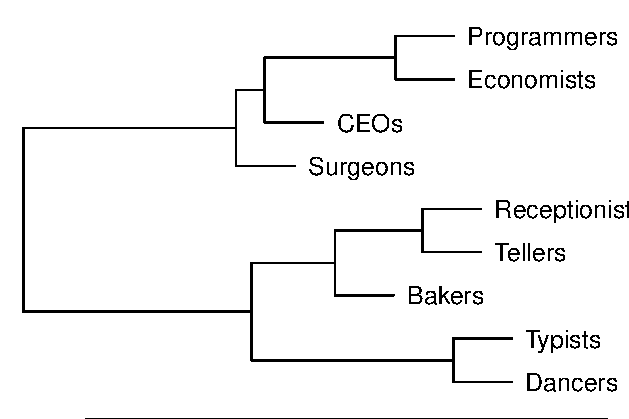
\includegraphics[width=\textwidth]{slides_fig/example_cluster.pdf} \\
  Hierarchical cluster analysis, work activity (Euclidean distance)
  \end{center}
\end{frame}

\begin{frame}
  \frametitle{O*NET Data Example: PCA}
  \begin{center}
  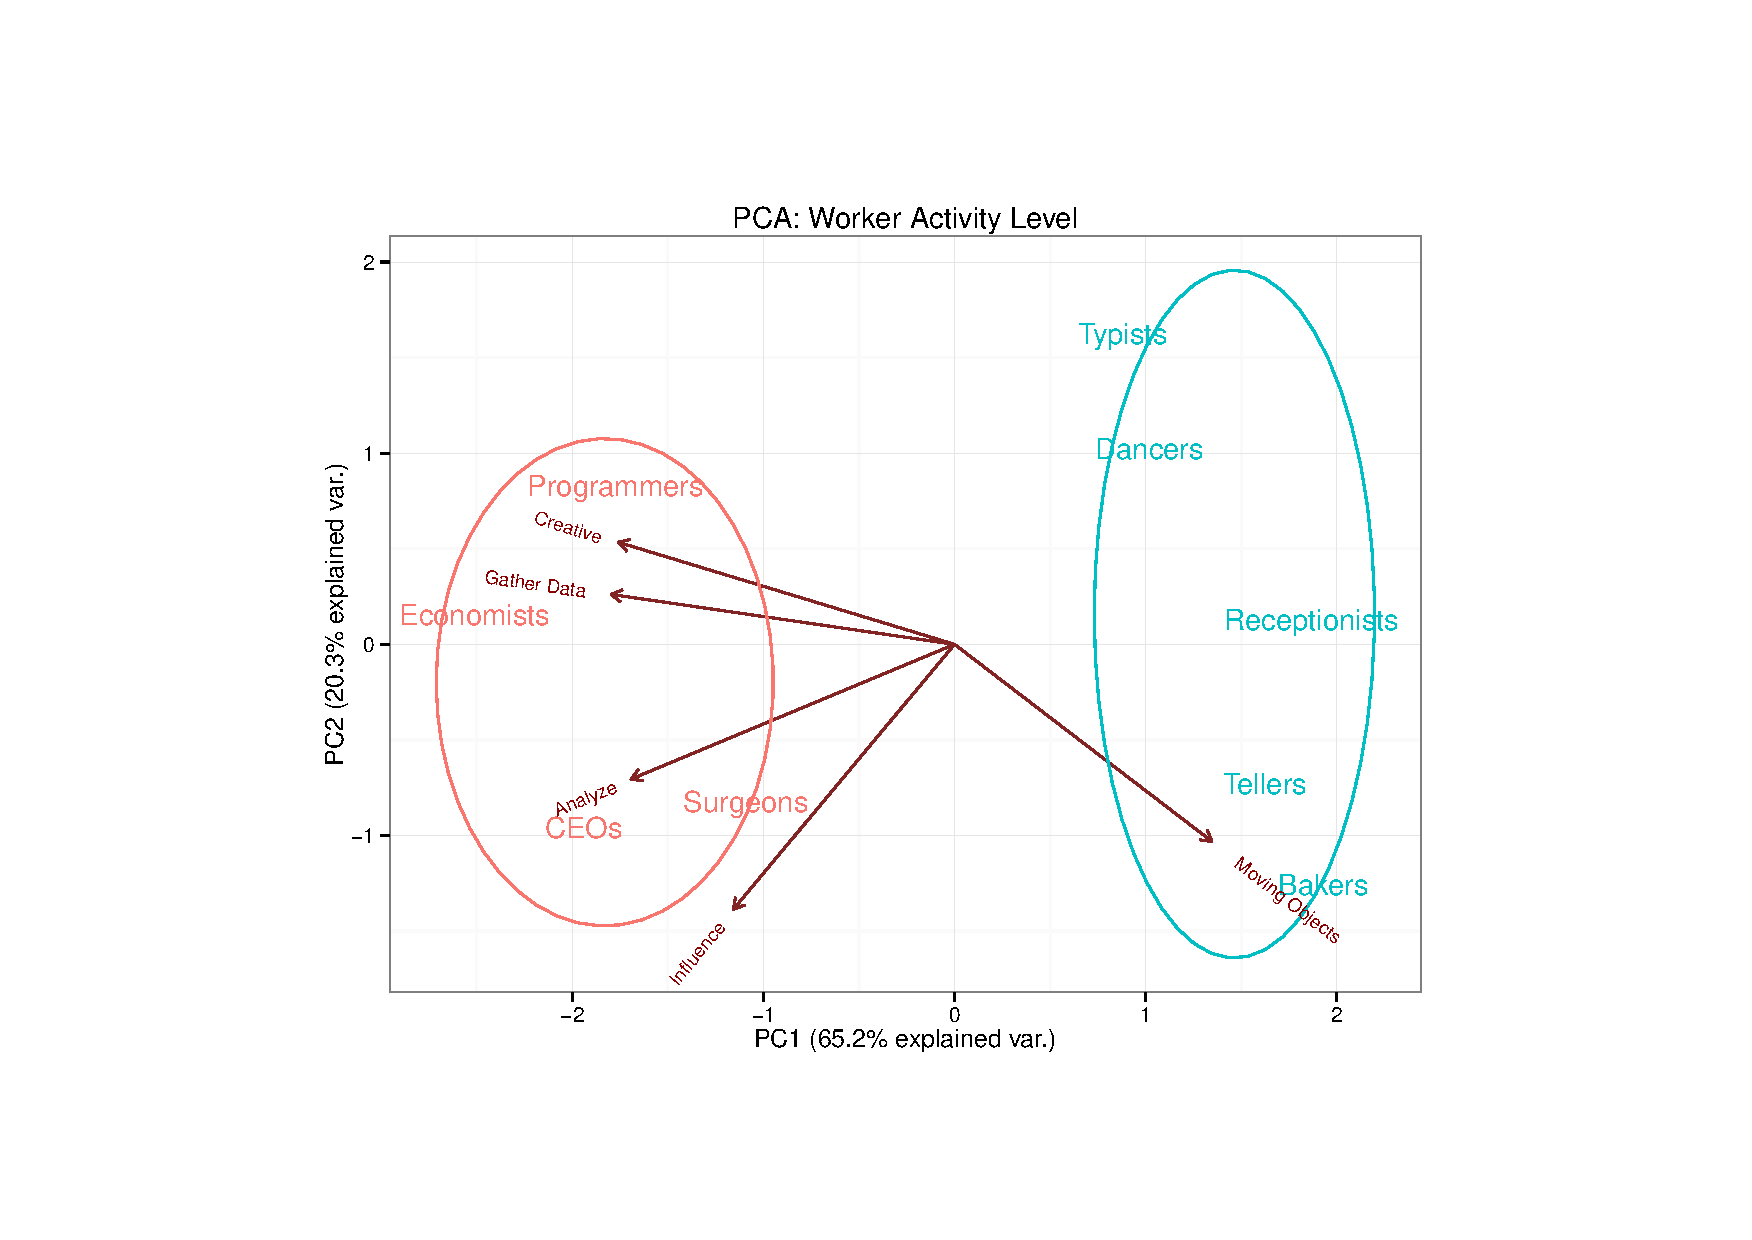
\includegraphics[width=0.8\textwidth]{slides_fig/pca_example.pdf} \\
  Groups identified with k-means cluster analysis (k=2).
  \end{center}
\end{frame}

\begin{frame}
  \frametitle{Identification Challenge}
  \begin{itemize}
  \item Employment is an outcome of supply and demand.
  \item But supply and demand curves are unobservable.
  \item However, wage quantiles {\em are} observable. 
%    As demand for a task falls, workers with lower comparative advantage switch tasks.
  \item \citet{Firpo2011} exploit quantile regression to analyze changes in labor demand.
  \end{itemize}
\end{frame}

\end{document} 
